\documentclass[10pt]{article}

% Packages and macros go here
\usepackage[T1]{fontenc}
\usepackage{lmodern}
\usepackage[utf8x]{inputenx}
\usepackage{microtype}
\usepackage{framed}
\usepackage{listings}
\usepackage{vmargin}
\usepackage{setspace}
\usepackage{mathrsfs, mathenv}
\usepackage{amsmath, amsthm, amssymb, amsfonts, amscd}
\usepackage{graphicx}
\usepackage{epstopdf}
\usepackage[svgnames]{xcolor}
\usepackage{hyperref}
\usepackage[capitalise]{cleveref}
\hypersetup{citecolor=blue, colorlinks=true, linkcolor=black}
\setlength{\parskip}{6pt}
\setlength\parindent{0pt}
\usepackage{subcaption}
\usepackage{bbm}
\usepackage{cite}
\usepackage{verbatim}
\usepackage{pgfplots}
\usepackage{tikz}
\usepackage{etoolbox}
\usepackage{color}
\usepackage{lipsum}
\usepackage{ifthen}
\usepackage[linesnumbered, ruled, vlined]{algorithm2e}
\crefname{algocf}{Algorithm}{Algorithms}
\usepackage{autonum}

\theoremstyle{plain}
\newtheorem{theorem}{Theorem}[section]
\newtheorem{corollary}[theorem]{Corollary}
\newtheorem{lemma}[theorem]{Lemma}
\newtheorem{proposition}[theorem]{Proposition}
\numberwithin{equation}{section}

\theoremstyle{definition}
\newtheorem{definition}[theorem]{Definition}

\theoremstyle{remark}
\newtheorem{remark}[theorem]{Remark}
\newtheorem{assumption}[theorem]{Assumption}
\newtheorem{example}[theorem]{Example}


\ifpdf
  \DeclareGraphicsExtensions{.eps,.pdf,.png,.jpg}
\else
  \DeclareGraphicsExtensions{.eps}
\fi

\usepackage{mathtools}
% basics

% tables
\usepackage{booktabs}

% plots
\usepackage{pgfplots}
\usepackage{tikz}
\usetikzlibrary{patterns,arrows,decorations.pathmorphing,backgrounds,positioning,fit,matrix}
\usepackage[labelfont=bf]{caption}
\setlength{\belowcaptionskip}{-5pt}
\usepackage{here}
\usepackage[font=normal]{subcaption}

% Prevent itemized lists from running into the left margin inside theorems and proofs
\usepackage{enumitem}
\setlist[itemize]{leftmargin=.5in}
\setlist[enumerate]{leftmargin=.5in,topsep=3pt,itemsep=3pt,label=(\roman*)}

% Add a serial/Oxford comma by default.
\newcommand{\creflastconjunction}{, and~}

% Sets running headers as well as PDF title and authors
% title and authors

\newcommand{\email}[1]{\href{#1}{#1}}
\newcommand{\TheTitle}{Probabilistic methods for elliptic partial differential equations} 
\newcommand{\TheAuthors}{A. Abdulle, G. Garegnani}
%\headers{Random time steps for quantifying chaotic numerical integration}{\TheAuthors}
\title{{\TheTitle}}
\newcommand*\samethanks[1][\value{footnote}]{\footnotemark[#1]}
\author{Assyr Abdulle\thanks{Institute of Mathematics, \'Ecole Polytechnique F\'ed\'erale de Lausanne (\email{\{assyr.abdulle, giacomo.garegnani\}@epfl.ch})}
	\and
	Giacomo Garegnani\samethanks}
\date{}

\usepackage{amsopn}
\DeclareMathOperator{\diag}{diag}
\DeclarePairedDelimiter{\ceil}{\left\lceil}{\right\rceil}
\DeclarePairedDelimiter{\floor}{\lfloor}{\rfloor}
\DeclarePairedDelimiter{\abs}{\lvert}{\rvert}
\DeclarePairedDelimiter{\norm}{\lVert}{\rVert}
\renewcommand{\phi}{\varphi}
\renewcommand{\theta}{\vartheta}
\renewcommand{\Pr}{\mathbb{P}}
\newcommand{\btilde}{\widetilde}
\newcommand{\bhat}{\widehat}
\newcommand{\eqtext}[1]{\ensuremath{\stackrel{#1}{=}}}
\newcommand{\leqtext}[1]{\ensuremath{\stackrel{#1}{\leq}}}
\newcommand{\iid}{\ensuremath{\stackrel{\text{i.i.d.}}{\sim}}}
\newcommand{\totext}[1]{\ensuremath{\stackrel{#1}{\to}}}
\newcommand{\rightarrowtext}[1]{\ensuremath{\stackrel{#1}{\longrightarrow}}}
\newcommand{\leftrightarrowtext}[1]{\ensuremath{\stackrel{#1}{\longleftrightarrow}}}
\newcommand{\pdv}[2]{\ensuremath\partial_{#2}#1}
\newcommand{\N}{\mathbb{N}}
\newcommand{\R}{\mathbb{R}}
\newcommand{\C}{\mathbb{C}}
\newcommand{\OO}{\mathcal{O}}
\newcommand{\epl}{\varepsilon}
\newcommand{\diffL}{\mathcal{L}}
\newcommand{\prior}{\mathcal{Q}}
\newcommand{\defeq}{\coloneqq}
\newcommand{\eqdef}{\eqqcolon}
\newcommand{\Var}{\operatorname{Var}}
\newcommand{\E}{\operatorname{\mathbb{E}}}
\newcommand{\MSE}{\operatorname{MSE}}
\newcommand{\trace}{\operatorname{tr}}
\newcommand{\MH}{\mathrm{MH}}
\newcommand{\ttt}{\texttt}
\newcommand{\Hell}{d_{\mathrm{H}}}
\newcommand{\sksum}{{\textstyle\sum}}
\newcommand{\dd}{\, \mathrm{d}}
\renewcommand{\d}{\mathrm{d}}
\definecolor{shade}{RGB}{100, 100, 100}
\definecolor{bordeaux}{RGB}{128, 0, 50}
\newcommand{\corr}[1]{{\color{red}#1}}
\newcommand{\Tau}{\tau}
\newcommand{\LL}{L}
\newcommand{\HH}{H}
\newcommand{\WW}{W}
\newcommand{\mbf}{\mathbf}
\newcommand{\bfs}{\boldsymbol}
\newcommand{\todo}{{\color{red} TO DO}}
\newcommand{\X}{\mathbb{X}}
\newcommand{\nablar}{\nabla_{\hat x}}
\newcommand{\eval}[1]{\bigr\rvert_{#1}}
\newcommand{\normm}[1]{\norm{#1}_a}
%\newcommand{\normm}[1]{{\left\vert\kern-0.25ex\left\vert\kern-0.25ex\left\vert #1 
%		\right\vert\kern-0.25ex\right\vert\kern-0.25ex\right\vert}}

\usepackage[usestackEOL]{stackengine}
\newcommand\fop[3][9pt]{\mathop{\ensurestackMath{\stackengine{#1}%
			{\displaystyle#2}{\scriptstyle#3}{U}{c}{F}{F}{L}}}\limits}
\newcommand\finf[2][9pt]{\fop[#1]{\inf}{#2}}
\newcommand\fsum[2][14pt]{\fop[#1]{\sum}{#2}}

\definecolor{leg1}{RGB}{0,114,189}
\definecolor{leg2}{RGB}{217,83,25}
\definecolor{leg3}{RGB}{237,177,32}
\definecolor{leg4}{RGB}{126,47,142}
\definecolor{leg5}{RGB}{119,172,48}

\definecolor{leg21}{RGB}{62,38,169}
\definecolor{leg22}{RGB}{46,135,247}
\definecolor{leg23}{RGB}{55,200,151}
\definecolor{leg24}{RGB}{254,195,56}


\ifpdf
\hypersetup{
	pdftitle={\TheTitle},
	pdfauthor={\TheAuthors}
}
\fi


\begin{document}
\maketitle	

\textbf{Abstract.}

\textbf{AMS subject classification.}

\textbf{Keywords.}

\section{Introduction}

\todo \cite{AbG20, KeH16, KSH18, CCC16, CGS17}

\begin{equation}\label{eq:ellipticEquation}
\begin{aligned}
	-\nabla \cdot (\kappa \nabla u) &= f, &&\text{in } D,\\
	u &= g, &&\text{on } \partial D.
\end{aligned}
\end{equation}

\textbf{important:} review of probabilistic methods for PDEs and ODEs. Have PDEs really been treated already? How? Inverse problems: what is the current state of things? Has anyone gone infinite dimensional?

\section{Notation and method}

\subsection{Notation}

We now introduce some basic notation which will be employed throughout this paper. Most of the notation is classic, but we report it here for completeness. The symbol $D \subset \R^2$ is employed for a bounded domain with smooth boundary, or for a convex polygon. The following symbols are employed for function spaces
\begin{itemize}
	\item $L^p(D) = \left\{v\colon D \to \R, \int_D v^p \dd x< \infty \right\}$,
	\item $W^{q, p}(D) = \left\{v \in L^p(D), \sum_{\abs{\alpha}\leq q} \abs{D^{\alpha} v} \in L^p(D) \right\}$,
	\item $H^q(D) \equiv W^{q,2}(D)$,
	\item $H^q_0(D) = \left\{v \in H^q(D), v\eval{\partial D} = 0\right\}$,
	\item $C^l_0(D) = \left\{v \in \mathcal C^l(D), v\eval{\partial D} = 0\right\}$.
\end{itemize}
For a function $v \in \mathcal X$ where $\mathcal X$ is any of the spaces above, we denote by $\norm{v}_{\mathcal X}$ and $\abs{v}_{\mathcal X}$ the usual norms and seminorms. Furthermore, for $L^p$ and $W^{q,p}$, the usual meaning is given for $p = \infty$. For a vector $x \in \R^2$ we denote simply by $\abs{x}$ its Euclidean norm. Moreover, we will employ the following symbols
\begin{itemize}
	\item $\mathcal T_h$ is a triangulation of $D$ satisfying \corr{assumption}, and $V_h$ is the space of linear finite elements with zero boundary conditions defined on $\mathcal T_h$,
	\item $\btilde{\mathcal T}_h$ is a perturbation of $\mathcal T_h$ as for \cref{def:RandomMesh} such that \cref{as:MeshPerturbation} holds, and $\btilde V_h$ is the space of linear finite elements with zero boundary conditions defined on $\btilde{\mathcal T}_h$.
\end{itemize}
Finally, if a function $v \colon D \to \R$ or $v \colon D \to \R^2$ is constant over a set $K \subset D$, we denote by $v\eval{K}$ its constant value.


\subsection{Method} 

Weak formulation: bilinear form $a\colon V\times V \to \R$ and a linear functional $F\colon V \to \R$ satisfying the usual continuity and coercivity constraints, look for $u \in V$ satisfying
\begin{equation}\label{eq:EXSol}
	a(u, v) = F(v),	
\end{equation}
for all functions $v \in V$. Galerkin formulation: for $V_h \subset V$ such that $\dim V_h < \infty$, find $u_h \in V_h$ such that
\begin{equation}\label{eq:FEMSol}
	a(u_h, v_h) = f(v_h), \quad \forall v_h \in V_h,
\end{equation}
for all $v_h \in V_h$. Given a triangulation $\mathcal T_h$ of the domain $D$, we choose $V_h$ to be the space of linear finite elements, i.e., $V_h = X_h^1 \cap V$, where 
\begin{equation}
	X_h^1 = \{v_h \in C^0(\overline D) \colon v_h|_{K} \in \mathcal P_1, \; \text{for all } K \in \mathcal T_h\},
\end{equation}
and where $\mathcal P_1$ is the space of polynomials of degree at most one. The finite element space can be written then as $V_h = \mathrm{span}\{\phi_i\}_{i=1}^N$, where the basis $\{\phi_i\}_{i=1}^N$ are the Lagrange basis functions. Hence, each $v_h \in V_h$ can be written as $v_h = \sum_{i=1}^N v_i \phi_i$, where $v_i$ are the coefficients of $v_h$ on the basis $\{\phi_i\}_{i=1}^N$. Our probabilistic method is based on a randomly perturbed mesh $\btilde {\mathcal T}_h$ which is defined as follows.

\begin{definition} \label{def:RandomMesh} Let us consider a domain $D \subset \R^d$ and a triangulation $\mathcal T_h$ characterised by the maximum diameter $h > 0$ of its elements and by the set of vertices $\mathcal N_h = \{x_i\}_{i=1}^{N}$ such that $\mathcal N_h = \mathcal N_h^I \cup \mathcal N_h^B$, where $\mathcal N_h^I$ and $\mathcal N_h^B$ are the vertices in the interior of $D$ and on $\partial D$ respectively, and where we denote $N_I = \abs{\mathcal N_h^I}$ and $N_B = \abs{\mathcal N_h^B}$. Given a probability space $(\Omega, \Sigma, \mu)$, the random mesh $\btilde {\mathcal T}_h$ is defined by a sequence of random variables $\{\alpha_i\}_{i=1}^{N_I}$, $\alpha_i \colon \Omega \to \R^d$, which are used to perturb the internal nodes as
	\begin{equation}
		\tilde x_i = x_i + h^p \alpha_i, \quad x_i \in \mathcal N_h^I,
	\end{equation}
	where $p \geq 1$. Let us remark that the vertices laying on $\partial D$ in $\mathcal T_h$ are unperturbed in $\btilde {\mathcal T}_h$.
\end{definition}

Once the perturbed mesh $\btilde {\mathcal T}_h$ is obtained, let us denote by $\btilde V_h$ the piecewise linear finite element space defined on $\btilde {\mathcal T}_h$. Let us remark that the space $\btilde V_h = \btilde V_h(\omega)$ is random itself, i.e., for each realisation of the random variables $\{\alpha_i\}_{i=1}^{N_I}$ we obtain a different perturbed finite element space.


\begin{definition} \label{def:ProbSolution} With the notation above, the probabilistic solution $\btilde u_h \colon \Omega \times D \to \R$ is a random field satisfying for all $\omega \in \Omega$
	\begin{equation}
		\btilde u_h(\omega, \cdot) \in \btilde V_h(\omega), \; \text{s.t. } a(\btilde u_h(\omega, \cdot), \btilde v_h) = F(\btilde v_h), \; \text{for all } \btilde v_h \in \btilde V_h(\omega). 
	\end{equation}
\end{definition}

Let us finally introduce the following assumption on the random variables defining the mesh perturbation. 
\begin{assumption} \label{as:MeshPerturbation} The random variables $\alpha_i$ satisfy
	\begin{equation}
		\abs{\alpha_i} \leq \frac12 \left(\frac{\rho_i}{h}\right)^p,
	\end{equation}
	almost surely, where
	\begin{equation}
		\rho_i = \min_{K \in \Delta(x_i)} \rho_K,
	\end{equation}
	with $\Delta(x_i)$ the set of all elements having $x_i$ as a vertex. With this choice, the topology of the mesh $\mathcal {\widetilde T}_h$ is almost surely the same as the topology of $\mathcal T_h$, i.e., the edges of $\mathcal {\widetilde T}_h$ do not cross.
\end{assumption}



\section{A priori error analysis}

In this section, we analyse the convergence a priori of our method. In particular, we wish the family of probabilistic solutions to be close to the solution obtained with the original mesh, i.e., we will prove that 
\begin{equation}\label{eq:DefProbConv}
	\norm{u_h - \btilde u_h}_{\mathcal X} \leq C\eta(h), \quad \text{a.s.},
\end{equation}
where $\eta \colon \R \to \R$ is such that $\eta(h) \to 0$ for $h \to 0$ and where $\mathcal X = \{H^1(D), L^\infty(D)\}$. Similarly to standard error analysis, we first introduce an interpolation result and then prove convergence in the above sense.

\subsection{Interpolation analysis}

In this section we consider the Legendre piecewise linear interpolants and their properties when they are employed to pass from the space $V_h$ to the space $\widetilde V_h$. Let us first recall the definition of the Legendre interpolant.

\begin{definition}\label{def:Legendre} Let $V = \mathcal C^0_0(D)$. We denote by $\Pi_h\colon V \to V_h$ and $\btilde \Pi_h\colon V \to \btilde V_h$ the Legendre piecewise linear interpolation operators on $V_h$ and $\btilde V_h$ respectively, i.e., for $v \in V$
	\begin{equation}
	\Pi_h v(x) = \fsum{x_j \in \mathcal N_h^I} v(x_j) \phi_j(x), \quad	\btilde \Pi_h v(x) = \fsum{\tilde x_j \in \btilde {\mathcal N}_h^I} v(x_j) \tilde \phi_j(x),
	\end{equation}
	where $\{\phi_i\}_{i=1}^{N^I}$ and $\{\tilde \phi_i\}_{i=1}^{N^I}$ are the basis functions of $V_h$ and $\btilde V_h$ respectively.
\end{definition}

In the following lemma we characterise the value that the Legendre interpolant $\btilde \Pi_h$ assumes on the nodes of the original mesh $\mathcal T_h$. Let us remark that $V_h \subset C_0^0(D)$, thus the interpolant above can be employed on $V_h$.

\begin{lemma}\label{lem:InterpPreliminary} With the notation of \cref{def:Legendre}, it holds for all $v_h \in V_h$ and all $x_i \in \mathcal N_h^I$
	\begin{equation}
	\begin{aligned}
		v_h(\tilde x_i) &= v_h(x_i) + \bar h_i^p \alpha_i^\top \nabla v_h(\tilde x_i), \\
		\btilde \Pi_h v_h(x_i) - v_h(x_i) &= \bar h_i^p \alpha_i^\top \Big(\nabla v_h(\tilde x_i) - \nabla \btilde \Pi_h v_h(x_i)\Big).
	\end{aligned}
	\end{equation}
\end{lemma}
\begin{proof} We can now expand the function $v_h$, which is linear on the segment connecting $x_i$ and $\tilde x_i$, as
	\begin{equation}\label{eq:TaylorVh}
	v_h(\tilde x_i) = v_h(x_i) + \bar h_i^p \alpha_i^\top \nabla v_h(\tilde x_i),
	\end{equation}
	which is the first equality. Let us now denote $e_h = \btilde \Pi_h v_h - v_h$. An exact Taylor expansion of the linear basis function $\tilde \phi_j$ gives
	\begin{equation}
	\begin{aligned}
	e_h(x_i) &= \sum_{j} v_h(\tilde x_j) \phi_j(x_i) - v_h(x_i) \\
	&= \sum_j v_h(\tilde x_j) \Big(\tilde \phi_j(\tilde x_i) - \bar h_i^p \alpha_i^\top \nabla \tilde \phi_j(x_i)\Big) - v_h(x_i) \\
	&= v_h(\tilde x_i) - v_h(x_i) - \sum_j \bar h_i^p \alpha_i^\top v_h(\tilde x_j) \nabla \tilde \phi_j(x_i).
	\end{aligned}
	\end{equation}
	This, together with \eqref{eq:TaylorVh}, yields
	\begin{equation}
	\begin{aligned}
	e_h(x_i) &= \bar h_i^p \alpha_i^\top \nabla v_h(\tilde x_i) - \bar h_i^p \alpha_i^\top \sum_j v_h(\tilde x_j) \nabla \tilde \phi_j(x_i) \\
	&= \bar h_i^p \alpha_i^\top \Big(\nabla v_h(\tilde x_i) - \nabla \btilde \Pi_h v_h(x_i)\Big),
	\end{aligned}
	\end{equation}
	which is the second desired equality and which therefore concludes the proof.
\end{proof}


We are not interested in all possible functions in $V_h$, but only in those which are close enough to a smooth function. The definition below sets the function space we consider in the following.

\begin{definition}\label{def:Vh2Inf} We denote by $V_h^{2, \infty} \subset V_h$ the space such that $v_h \in V_h^{2, \infty}$ if there exists $v \in W^{2, \infty}(D)$ satisfying
	\begin{equation}
		\norm{v - v_h}_{W^{1, \infty}(D)} \leq C h \abs{\log h} \abs{v}_{W^{2, \infty}(D)},
	\end{equation} 
	where $C > 0$ is a constant independent of $h$.
\end{definition}

In the following Lemma, we provide a property of functions in $V_h^{2, \infty}$ which is quite consequent from the definition of the space. Since we repeatedly employ this result in the following, let us highlight it here.
\begin{lemma}\label{lem:Vh2InfPropr} Let $v_h \in V_h^{2, \infty}$. Then, if two triangles $K, K' \in \mathcal T_h$ share a vertex, it holds
	\begin{equation}
		\abs{\nabla v_h \eval{K} - \nabla v_h \eval{K'}} \leq Ch \abs{\log h} \abs{v}_{W^{2, \infty}(D)},
	\end{equation} 
	for a constant $C > 0$ independent of $h$.
\end{lemma}
\begin{proof} The proof follows from the triangle inequality. In particular, let $x \in K$ and $x' \in K'$. Then, there exists $v \in W^{2, \infty}$ such that
	\begin{equation}
	\begin{aligned}
		\abs{\nabla v_h \eval{K} - \nabla v_h \eval{K'}} &\leq \abs{\nabla v_h \eval{K} - \nabla v(x)} + \abs{\nabla v_h \eval{K'} - \nabla v (x')} + \abs{\nabla v (x) - \nabla v (x')}\\
		&\leq 2 \abs{v_h - v}_{W^{1, \infty}(D)} + \abs{v}_{W^{2, \infty}(D)}\abs{x - x'}.
	\end{aligned}
	\end{equation}
	The desired result follows from the definition of $V_h^{2, \infty}$ and from the fact that since $K$ and $K'$ share a vertex, it is possible to bound $\abs{x - x'} \leq Ch$.
\end{proof}

In the following we consider the affine maps which define locally the geometry of the mesh. Let $K \in \mathcal T_h$ be an element of the original mesh, and $\btilde K \in \widetilde{\mathcal T}_h$ be the corresponding element in the perturbed mesh. Moreover, let us denote by $x_1, x_2, x_3$ the vertices of $K$ and by $\tilde x_1, \tilde x_2, \tilde x_3$ the corresponding vertices of $\btilde K$. We denote by $\bhat K$ the reference element, i.e., the triangle with vertices $\hat x_1 = (0, 0)^\top$, $\hat x_2 = (1, 0)^\top$, $\hat x_3 = (0, 1)^\top$. We consider the affine maps $F_K \colon \bhat K \to K$ and $\btilde F_K \colon \bhat K \to \btilde K$ defined for all $\bhat x \in \bhat K$ as 
\begin{equation}
F_K(\hat x) = B_K\hat x + b_K, \quad \btilde F_K(\hat x) = \btilde B_K\hat x + \tilde b_K,
\end{equation}
where $b_K = x_1$, $\tilde b_K = \tilde x_1$ and the matrices $B_K, \btilde B_K \in \R^{2\times 2}$ are defined as
\begin{equation}
B_K = \begin{pmatrix} x_2 - x_1 \mid x_3 - x_1 \end{pmatrix}, \quad B_{\btilde K} = \begin{pmatrix} \tilde x_2 - \tilde x_1 \mid \tilde x_3 - \tilde x_1\end{pmatrix},
\end{equation}
so that $F_K(\bhat x_i) = x_i$ and $\btilde F_K(\bhat x_i) = \tilde x_i$ for $i = 1, 2, 3$. The ``closeness'' of $K$ to $\widetilde K$ can be studied in terms of the matrices $B_K$ and $\widetilde B_K$, and the relation linking these two matrices is given in the following Lemma.
\begin{lemma}\label{lem:ReferenceMaps} Let \cref{as:MeshPerturbation} hold. If $K \in \mathcal T_h$ and $\btilde K \in \btilde{\mathcal T}_h$ is the corresponding element in the perturbed mesh, then
	\begin{equation}
		B_{\btilde K}^{-\top} - B_K^{-\top} = \Gamma,
	\end{equation}
	where the matrix $\Gamma \in \R^{2 \times 2}$ satisfies $\abs{\Gamma} \leq C$ a.s. for a constant $C > 0$ independent of $h$ and is given by the infinite sum
	\begin{equation}\label{eq:DefGammaMatrix}
		\Gamma = \sum_{j=1}^\infty (-1)^j \left(h^p \Lambda^\top B_K^{-\top}\right)^j, \quad \text{with } \Lambda = \begin{pmatrix} \alpha_2 - \alpha_1 \mid \alpha_3 - \alpha_1 \end{pmatrix}.
	\end{equation}
\end{lemma}
\begin{proof} From the definition of $\btilde K$ and under \cref{as:MeshPerturbation}, it is clear that $\btilde B_K = B_K + h^p\Lambda$. Moreover, we can rewrite $B_{\btilde K}^{-\top}$ with algebraic operations as
\begin{equation}
	B_{\btilde K}^{-\top} = (B_K + h^p \Lambda)^{-\top} = B_K^{-\top}(I + h^p B_K^{-1}\Lambda)^{-\top}.
\end{equation}
In order for the final result to hold, we need that
\begin{equation}\label{eq:DefGammaMatrix_2}
	(I + h^p B_K^{-1}\Lambda)^{-\top} = I + \Gamma,
\end{equation}
with $\Gamma$ given in \eqref{eq:DefGammaMatrix}. This is true whenever $h^p \abs{B_K^{-1} \Lambda} < 1$. Denoting by $\bhat h$ the exterior diameter of the reference triangle $\bhat K$ and applying \cite[Theorem 3.1.3]{Cia02} we have
\begin{equation}
	\abs{B_K^{-1} \Lambda} \leq \abs{B_K^{-1}}\abs{\Lambda} \leq \frac{\bhat h}{\rho_K} \abs{\Lambda}.
\end{equation}
Let us now remark that due to \cref{as:MeshPerturbation}, it holds
\begin{equation}
	\abs{\Lambda}^2 \leq 2 \abs{\alpha_1}^2 + \abs{\alpha_2}^2 + \abs{\alpha_3}^2 \leq \left(\frac{\rho_K}{h^p}\right)^2, \quad \text{a.s.},
\end{equation}
which implies $h^p\abs{B_K^{-1} \Lambda} \leq \bhat h$ a.s. Now $\bhat h = 1 / \sqrt{2}$, so we have that $h^p\abs{B_K^{-1}\Lambda} < 1$ a.s. and therefore the series \eqref{eq:DefGammaMatrix} converges.
\end{proof}

We now proceed to bound the difference between the gradient of $v_h$ and of its interpolant $\widetilde \Pi_h v_h$ on a single element. 

\begin{lemma}\label{lem:Interp_BoundKKTilde} With the notation of \cref{def:RandomMesh}, \cref{def:Legendre} and \cref{lem:ReferenceMaps}, it holds for all $v_h \in V_h^{2, \infty}$
	\begin{equation}
		\abs{\nabla v_h\eval{K} - \nabla \btilde \Pi_h v_h \eval{\btilde K}} \leq C h^p \abs{\log h} \abs{v}_{\WW^{2, \infty}(D)},
	\end{equation}
	where $p$ is given in \cref{def:RandomMesh}.
\end{lemma}
\begin{proof} Let us define $\bhat v_h \colon \bhat K \to \R$ as $\bhat v_h \defeq v_h \circ F_K$ and $\btilde \Pi_h \bhat v_h\colon \bhat K \to \R$ as $\btilde \Pi_h \bhat v_h \defeq \btilde \Pi_h v_h \circ \btilde F_K$. Then, the chain rule yields
\begin{equation}\label{eq:DiffMapToRef}
	\nabla v_h\eval{K} - \nabla \btilde \Pi_h v_h \eval{\btilde K} = B_K^{-\top} \bhat \nabla \bhat v_h - B_{\btilde K}^{-\top} \bhat \nabla \btilde \Pi_h \bhat v_h,
\end{equation}
where $\bhat \nabla$ is the gradient with respect to $\hat x$. Moreover, the gradient on the reference triangle of the interpolated function satisfies
\begin{equation}
	\bhat\nabla \btilde \Pi_h \bhat v_h = \begin{pmatrix} \btilde \Pi_h \bhat v_h(\hat x_2) - \btilde \Pi_h \bhat v_h(\hat x_1) \\
													 \btilde \Pi_h \bhat v_h(\hat x_3) - \btilde \Pi_h \bhat v_h(\hat x_1) \end{pmatrix}
								   = \begin{pmatrix} \btilde \Pi_h v_h(\tilde x_2) - \btilde \Pi_h v_h(\tilde x_1) \\
								   					 \btilde \Pi_h v_h(\tilde x_3) - \btilde \Pi_h v_h(\tilde x_1) \end{pmatrix}.
\end{equation}
Since the interpolation is exact on the nodes of the mesh $\btilde{\mathcal T}_h$ and due to \cref{lem:InterpPreliminary}, this yields
\begin{equation}
	\bhat\nabla \btilde \Pi_h \bhat v_h = \begin{pmatrix} v_h(\tilde x_2) - v_h(\tilde x_1) \\
													 v_h(\tilde x_3) - v_h(\tilde x_1) \end{pmatrix}
								   = \begin{pmatrix} v_h(x_2) - v_h(x_1) \\
								   					 v_h(x_3) - v_h(x_1) \end{pmatrix} + h^p \gamma
								   = \bhat \nabla \bhat v_h + h^p \gamma,
\end{equation}
where 
\begin{equation}
	\gamma = \begin{pmatrix} \alpha_2^\top \nabla v_h(\tilde x_2) - \alpha_1^\top \nabla v_h(\tilde x_1) \\
			 				 \alpha_3^\top \nabla v_h(\tilde x_3) - \alpha_1^\top \nabla v_h(\tilde x_1) \end{pmatrix}.
\end{equation}
Employing \cref{lem:ReferenceMaps}, we can replace the expression for $B_{\btilde K}$ in \eqref{eq:DiffMapToRef} and deduce
\begin{equation}\label{eq:SumExpansionGradGradTilde}
	\nabla v_h\eval{K} - \nabla \btilde \Pi_h v_h \eval{\btilde K} = -B_K^{-\top}\left(h^p(I + \Gamma)\gamma + \Gamma \bhat \nabla \bhat v_h \right).
\end{equation}
Let us now remark that from \eqref{eq:DefGammaMatrix_2} $\Gamma$ satisfies 
\begin{equation}
	\Gamma = -(I + \Gamma)h^p\Lambda^\top B_K^{-\top},
\end{equation}
which together with \eqref{eq:SumExpansionGradGradTilde} yields
\begin{equation}\label{eq:SumExpansionGradGradTilde_2}
	\nabla v_h\eval{K} - \nabla \btilde \Pi_h v_h \eval{\btilde K} = h^p B_K^{-\top}(I + \Gamma)\left(\lambda^\top B_K^{-\top} \bhat \nabla \bhat v_h - \gamma\right).
\end{equation}
We can now compute explicitly 
\begin{equation}
\begin{aligned}
	\gamma - \Lambda^\top B_K^{-\top} \bhat \nabla \bhat v_h &= \gamma - \Lambda^\top \nabla v_h \eval{K} \\
	&= \begin{pmatrix}  \alpha_2^\top \nabla v_h(\tilde x_2) - \alpha_1^\top \nabla v_h(\tilde x_1) \\
						\alpha_3^\top \nabla v_h(\tilde x_3) - \alpha_1^\top \nabla v_h(\tilde x_1) \end{pmatrix}
	- \begin{pmatrix} (\alpha_2^\top - \alpha_1^\top) \nabla v_h \eval{K} \\ 
					  (\alpha_3^\top - \alpha_1^\top) \nabla v_h \eval{K} \end{pmatrix} \\
	&= \begin{pmatrix} \alpha_2^\top \big(\nabla v_h(\tilde x_2) - \nabla v_h \eval{K}\big) + \alpha_1^\top \big(\nabla v_h \eval{K} - \nabla v_h(\tilde x_1)\big) \\
					   \alpha_3^\top \big(\nabla v_h(\tilde x_3) - \nabla v_h \eval{K}\big) + \alpha_1^\top \big(\nabla v_h \eval{K} - \nabla v_h(\tilde x_1)\big) \end{pmatrix}.                
\end{aligned}
\end{equation}	
Due to \cref{lem:Vh2InfPropr} and \cref{as:MeshPerturbation} we have therefore
\begin{equation}
	\abs{\gamma - \Lambda^\top B_K^{-\top} \bhat \nabla \bhat v_h} \leq Ch \abs{\log h}\abs{v}_{W^{2, \infty}(D)},
\end{equation}
almost surely, which, together with \eqref{eq:SumExpansionGradGradTilde_2}, implies 
\begin{equation}
	\abs{\nabla v_h\eval{K} - \nabla \btilde \Pi_h v_h \eval{\btilde K}} \leq Ch^{p+1}\abs{\log h}\abs{v}_{\WW^{2, \infty}(D)} \abs{B_K^{-\top}} \abs{I + \Gamma}
\end{equation}
Finally, since $\abs{B_K^{-1}} \leq Ch^{-1}$ and due to Lemma \ref{lem:ReferenceMaps}, we obtain
\begin{equation}
	\abs{\nabla v_h\eval{K} - \nabla \btilde \Pi_h v_h \eval{\btilde K}} \leq C h^p \abs{\log h} \abs{v}_{\WW^{2, \infty}(D)},
\end{equation}
which is the desired result.
\end{proof}

We can now prove an interpolation result in $L^\infty(D)$
\begin{lemma}\label{lem:Interp2D_Linf} With the notation of \cref{def:Vh2Inf}, let $v_h \in V_h^{2, \infty}$. Then, with the notation of \cref{def:Legendre}, it holds
		\begin{equation}
		\norm{v_h - \btilde \Pi_h v_h}_{L^\infty(D)} \leq Ch^{p+1} \abs{\log h},
		\end{equation}
		where $C > 0$ is a constant independent of $h$. 
\end{lemma}
\begin{figure}[t]
	\centering
	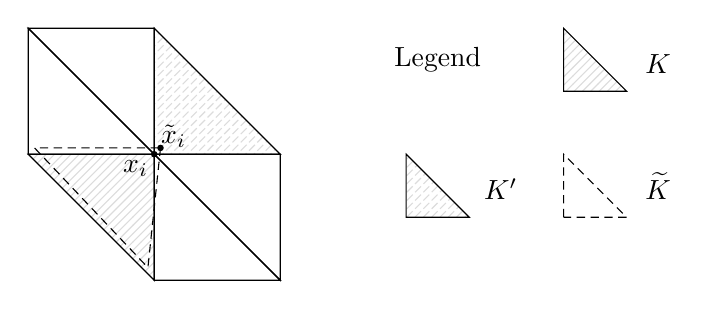
\begin{tikzpicture}[scale=0.8]
	% Pattern of triangles
	\draw[preaction={clip, postaction={pattern=north east lines, pattern color= {rgb,255:red,220; green,220; blue,220}}}] (2,2) -- (2,0) -- (0,2) -- cycle;
	\draw (2,2) -- (2,0) -- (4,0) -- cycle;
	\draw (2,2) -- (0,2) -- (0,4) -- cycle;
	\draw (2,2) -- (2,4) -- (0,4) -- cycle;
	\draw[preaction={clip, postaction={pattern=north east lines, dashed, pattern color= {rgb,255:red,220; green,220; blue,220}}}] (2,2) -- (2,4) -- (4,2) -- cycle;
	\draw (2,2) -- (4,2) -- (4,0) -- cycle;
	% Modified triangles
	\draw[densely dashed] (2.1,2.1) -- (1.9, 0.2) -- (0.1, 2.1) -- cycle;
	% Points
	\node[anchor = north east, inner sep = 2pt] at (2, 2) (xi) {$x_i$}; 
	\node[anchor = south west, inner sep = 0] at (2.1, 2.1) (xitilde) {$\tilde x_i$};
	\draw[fill=black] (2,2) circle[radius=1.2pt];
	\draw[fill=black] (2.1,2.1) circle[radius=1.2pt];
	% Legend
	\node at (6.5, 3.5) (leg) {Legend}; 
	\draw[preaction={clip, postaction={pattern=north east lines, pattern color= {rgb,255:red,220; green,220; blue,220}}}] (8.5,3) -- (8.5,4) -- (9.5,3) -- cycle;
	\node at (10,3.5) (legK) {$\vphantom{\btilde K}K$};
	\draw[preaction={clip, postaction={pattern=north east lines, dashed, pattern color= {rgb,255:red,220; green,220; blue,220}}}] (6,1) -- (6,2) -- (7,1) -- cycle;
	\node at (7.5,1.5) (legK2) {$\vphantom{\btilde K} K'$};
	\draw[densely dashed] (8.5,1) -- (8.5,2) -- (9.5,1) -- cycle;
	\node at (10,1.5) (legKtilde) {$\btilde K$};
	\end{tikzpicture}
	\caption{Scheme for the proof of Lemma \ref{lem:Interp2D_Linf}. The triangle with solid grey lines on the background is $K$, the triangle with dashed grey lines on the background is $K'$ and the triangle with dashed borders is $\btilde K$.}
	\label{fig:Error2D}
\end{figure}
\begin{proof} Let us denote $e_h = \btilde \Pi_h v_h - v_h$ and let us consider $x_i \in \mathcal N^I$. By definition $e_h(\tilde x_i) = 0$ for all $i = 0, \ldots, N$ and due to \cref{lem:InterpPreliminary}
	\begin{equation}\label{eq:ValueNodes}
		e_h(x_i) = h^p \alpha_i \big(\nabla v_h(\tilde x_i) - \nabla \btilde \Pi_hv_h(x_i)\big)  \eqdef h^p \alpha_i\epl_i.
	\end{equation}
	Let us denote by $K$ the element of $\mathcal T_h$ such that the corresponding element $\btilde K \in \widetilde{\mathcal T}_h$ contains $x_i$. Furthermore, let us denote by $K'$ the element in the original mesh containing $\tilde x_i$. We refer to \cref{fig:Error2D} for a schematic representation of these elements. With this notation, we have 
	\begin{equation}
		\nabla v_h(\tilde x_i) = \nabla v_h\eval{K'}, \quad \nabla \btilde \Pi_hv_h(x_i) = \nabla \btilde \Pi_h v_h\eval{\btilde K},
	\end{equation}
	and we can then decompose $\epl_i$ as $\epl_i = \epl_{i,1} + \epl_{i, 2}$ with
	\begin{equation}
		\epl_{i, 1} = \nabla v_h\eval{K'} - \nabla v_h\eval{K}, \quad  \epl_{i, 2} = \nabla v_h\eval{K}  - \nabla \btilde \Pi_h v_h \eval{\btilde K}.
	\end{equation}
	Due to \cref{lem:Vh2InfPropr}, we have 
	\begin{equation}\label{eq:boundEps1Proof2d}
	\abs{\epl_{i, 1}} \leq C h \abs{\log h} \abs{v}_{W^{2, \infty}(D)},
	\end{equation}
	Moreover, due to \cref{lem:Interp_BoundKKTilde}, we have
	\begin{equation}
		\abs{\epl_{i, 2}} \leq C h^p \abs{\log h} \abs{v}_{W^{2, \infty}(D)}
	\end{equation} 
	Since $p \geq 1$, the triangular inequality yields $\epl_{i} \leq Ch \abs{\log h} \abs{v}_{\WW^{2, \infty}(D)}$ for each node. Replacing this bound in \eqref{eq:ValueNodes}, we get for each $x_i \in \mathcal N_h^I$
	\begin{equation}
		\abs{e_h(x_i)} \leq C h^{p+1} \alpha_i \abs{\log h} \abs{v}_{\WW^{2, \infty}(D)}.
	\end{equation}
	Let us now remark that since by definition $e_h(\tilde x_i) = 0$ for all modified nodes, and since $e_h$ is linear on $D$, the maximum of $e_h$ has to be realised on one of the nodes of the original mesh. Hence
	\begin{equation}
		\norm{e_h}_{\LL^{\infty}(D)} = \max_{x_i \in \mathcal N_h^{I}} \abs{e_h(x_i)} \leq C h^{p+1} \abs{\log h} \abs{v}_{\WW^{2, \infty}(D)},
	\end{equation}
	which implies the desired result.
\end{proof}

We now consider the interpolation error in $H^1(D)$.
\begin{lemma}\label{lem:Interp2D_H1} With the notation of \cref{def:Vh2Inf}, let $v_h \in V_h^{2, \infty}$. Then, with the notation of \cref{def:Legendre}, it holds
	\begin{equation}
		\norm{v_h - \btilde \Pi_h v_h}_{\HH^1(D)} \leq Ch^{(p+1)/2} \abs{\log h},
	\end{equation}
	where $C > 0$ is a constant independent of $h$. 
\end{lemma}
\begin{figure}[t]
	\centering
	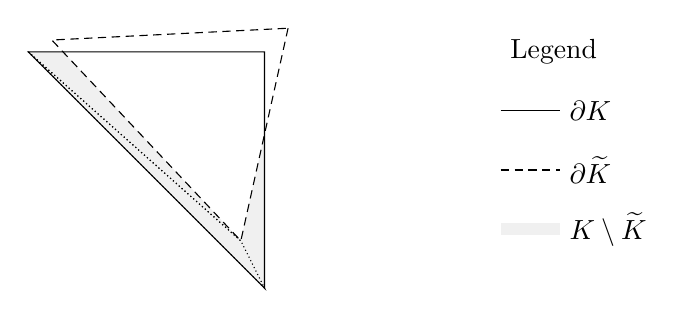
\begin{tikzpicture}[scale=1.5]
	% fill first
	\fill[fill={rgb,255:red,240; green,240; blue,240}] (0,2) -- (1.8, 0.4) -- (0.295,2) -- cycle;
	\fill[fill={rgb,255:red,240; green,240; blue,240}] (0,2) -- (1.8, 0.4) -- (2,0) -- cycle;
	\fill[fill={rgb,255:red,240; green,240; blue,240}] (2,1.3) -- (1.8, 0.4)  -- (2,0) -- cycle;
	% Pattern of triangles
	\draw[] (2,2) -- (2,0) -- (0,2) -- cycle;
	% Modified triangles
	\draw[densely dashed] (2.2,2.2) -- (1.8, 0.4) -- (0.2, 2.1) -- cycle;
	% Mini triangles
	\draw[densely dotted] (0,2) -- (1.8, 0.4) -- (2,0) -- cycle;
	\draw[densely dotted] (0,2) -- (1.8, 0.4); 
	% Legend
	\node[anchor = west] at (4, 2) (leg) {Legend};
	\draw[] (4, 1.5) -- (4.5, 1.5);
	\node[anchor = west] at (4.5, 1.5) (xi) {$\partial K$}; 
	\draw[densely dashed] (4, 1) -- (4.5, 1);
	\node[anchor = west] at (4.5, 1) (xi) {$\partial \widetilde K$}; 
	\fill[fill={rgb,255:red,240; green,240; blue,240}] (4, 0.55) -- (4.5, 0.55) -- (4.5, 0.45) -- (4, 0.45) -- cycle;
	\node[anchor = west] at (4.5, 0.5) (KmK) {$K \setminus \widetilde K$};
	\end{tikzpicture}
	\caption{Scheme for the proof of \cref{lem:Interp2D_H1}. The triangle with solid border is $K \in \mathcal T_h$, the one with dashed border is $\widetilde K \in \widetilde T_h$. The area filled in grey is $K \setminus \widetilde K$, and the dotted lines give one of the possible subdivision in triangles of $K \setminus \widetilde K$.}
	\label{fig:Error2D_H1}
\end{figure}
\begin{proof} First, let us recall that for any triangle of sides of length $a, b, c$ and of area $A$ it holds \cite{CuB67}
	\begin{equation}\label{eq:TriangleInequality}
		A \leq \frac{4\sqrt{3}}{9} \frac{abc}{a+b+c}.
	\end{equation}
	Let us now consider an element $K \in \mathcal T_h$ and the corresponding element $\widetilde K \in \widetilde{\mathcal T}_h$. It is clear (see e.g. \cref{fig:Error2D_H1}) that it is possible to subdivide $K \setminus \widetilde K$ into a bounded number of triangles for which the length one side is bounded by $Ch^p$ and the length of the two other side is bounded by $Ch$. Therefore, due to \eqref{eq:TriangleInequality} we have
	\begin{equation}\label{eq:AreaKMinusKTilde}
		\abs{K \setminus \widetilde K} \leq C \frac{h^{p+2}}{h + h + h^p} \leq Ch^{p+1}.
	\end{equation}
	Moreover, we remark that
	\begin{equation}\label{eq:AreaKIntersKTilde}
		\abs{K \cap \widetilde K} \leq \abs{K} \leq Ch^2.
	\end{equation}
	Let us now denote by $N_K$ the number of triangles in which the set $K\setminus \widetilde K$ is divided and by $K_{\mathrm{diff}}^{(i)}$, $i= 1, \ldots, N_K$ these triangles. We have
	\begin{equation}
		\int_K \abs{\nabla e_h}^2 \dd x = \int_{K \cap \widetilde K} \abs{\nabla  e_h}^2 \dd x+ \sum_{i=1}^{N_K} \int_{K_{\mathrm{diff}}^{(i)}}\abs{\nabla  e_h}^2 \dd x.
	\end{equation}
	Now, \cref{lem:Interp_BoundKKTilde} and \eqref{eq:AreaKIntersKTilde} yield
	\begin{equation}\label{eq:IntegralKIntersKTilde}
		\int_{K \cap \widetilde K} \abs{\nabla  e_h}^2 \dd x = \int_{K \cap \widetilde K} \abs{\nabla v_h\eval{K} - \nabla \btilde \Pi_h v_h \eval{\btilde K}}^2 \dd x \leq C h^{2p+2} \abs{\log h}^2 \abs{v}_{\WW^{2, \infty}(D)}^2.
	\end{equation}
	Let us now consider the second term. Each triangle $K_{\mathrm{diff}}^{(i)}$ intersects a finite number $N_K^{(i)}$ of triangles in the mesh $\widetilde{\mathcal T}_h$. We denote by $\widetilde K^{(i,j)}$ for $j = 1, \ldots, N_K^{(i)}$ these triangles and by $\widetilde K^{(i,j)}_{\mathrm{diff}} = \widetilde K^{(i,j)} \cap \widetilde K^{(i)}_{\mathrm{diff}}$, for which we remark that it holds
	\begin{equation}
		\abs{\widetilde K_{\mathrm{diff}}^{(i,j)}}\leq\abs{K_{\mathrm{diff}}^{(i)}}\leq\abs{K\setminus\widetilde K} \leq Ch^{p+1}.
	\end{equation}
	Finally, for each $i,j$ we denote by $K^{(i,j)}$ the element of $\mathcal T_h$ corresponding to $\widetilde K^{(i,j)} \in \mathcal T_h$ and remark that it is a neighbour of $K$. Therefore
	\begin{equation}
		\int_{K_{\mathrm{diff}}^{(i)}}\abs{e_h}^2 \dd x = \sum_{j=1}^{N_K^{(i)}} \int_{\widetilde K_{\mathrm{diff}}^{(i,j)}}\abs{e_h}^2 \dd x,
	\end{equation}
	where due to Young's inequality we have 
	\begin{equation}\label{eq:BoundLocalProof2D}
	\begin{aligned}
		\int_{\widetilde K_{\mathrm{diff}}^{(i,j)}}\abs{\nabla  e_h}^2 \dd x &= \int_{\widetilde K_{\mathrm{diff}}^{(i,j)}} \abs{\nabla v_h\eval{K} - \nabla \widetilde \Pi_h v_h\eval{\widetilde K^{(i,j)}}}^2 \dd x \\
		&\leq 2\left(\abs{\nabla v_h\eval{K} - \nabla v_h\eval{K^{(i,j)}}}^2 + \abs{\nabla \widetilde \Pi_h v_h\eval{\widetilde K^{(i,j)}} - \nabla v_h\eval{K^{(i,j)}}}^2\right) \abs{\widetilde K_{\mathrm{diff}}^{(i,j)}}.
	\end{aligned}
	\end{equation}
	Due to \cref{lem:Vh2InfPropr}, we have first
	\begin{equation}
		\abs{\nabla v_h\eval{K} - \nabla v_h\eval{K^{(i,j)}}}^2 \leq C h^2 \abs{\log h}^2 \abs{v}_{\WW^{2, \infty}(D)}^2,
	\end{equation}
	and due to \cref{lem:Interp_BoundKKTilde}, we obtain
	\begin{equation}
		\abs{\nabla \widetilde \Pi_h v_h\eval{\widetilde K^{(i,j)}} - \nabla v_h\eval{K^{(i,j)}}}^2 \leq C h^{2p} \abs{\log h}^2 \abs{v}_{\WW^{2, \infty}(D)}^2.
	\end{equation}
	Therefore, replacing these two inequalities and \eqref{eq:AreaKMinusKTilde} in \eqref{eq:BoundLocalProof2D} and since $p\geq 1$ and $h < 1$, we obtain for a constant $C > 0$
	\begin{equation}
		\int_{\widetilde K_{\mathrm{diff}}^{(i,j)}}\abs{\nabla  e_h}^2 \dd x \leq C h^{p+3} \abs{\log h}^2 \abs{v}_{\WW^{2, \infty}(D)}^2.
	\end{equation}
	Hence, we get
	\begin{equation}\label{eq:IntegralKMinusKTilde}
		\int_{K \setminus \widetilde K} \abs{\nabla  e_h}^2 \dd x\leq C N_K \left(\sum_{i=1}^{N_K} N_K^{(i)} \right)h^{p+3} \left(\abs{\log h} + 1\right)^2 \abs{v}_{\WW^{2, \infty}(D)}^2.
	\end{equation}
	Combining \eqref{eq:IntegralKIntersKTilde} and \eqref{eq:IntegralKMinusKTilde} and since $2p+2\geq p+3$ for $p \geq 1$, we conclude that there exists a constant $C > 0$ independent of $h$ but dependent on $v$ such that
	\begin{equation}
		\int_K \abs{\nabla  e_h}^2 \dd x \leq Ch^{p+3}\abs{\log h}^2.
	\end{equation}
	Finally, due to \corr{assumption on the mesh}, we have that $N \leq Ch^2$ and therefore
	\begin{equation}
		\abs{e_h}_{H^1(D)}^2 = \sum_{K \in \mathcal T_h} \int_K \abs{\nabla  e_h}^2 \dd x \leq Ch^{p+1}\abs{\log h}^2,
	\end{equation}
	which implies the desired result.
\end{proof}

\subsection{The sum space}

In order to prove convergence of the probabilistic solution, and moreover the closeness of $u_h$ to $\btilde u_h$ in the sense of \eqref{eq:DefProbConv}, we first need to define a convenient function space which is finite dimensional but which contains both $V_h$ and $\btilde V_h$. 

\begin{definition} Let us denote by $V_h^+ \subset V$  the space of functions that can be written as the sum of a function in $V_h$ and a function in $\btilde V_h$, i.e., for any function $v_h^+ \in V_h^+$ there exists functions $v_h \in V_h$ and $\btilde v_h \in \btilde V_h$ such that $v_h^+ = v_h + \btilde v_h$. 
\end{definition}

\begin{remark} Let us remark that in our setting of homogeneous boundary conditions $V_h \cap \btilde V_h = \{0\}$ almost surely. Therefore, the space $V_h^+$ is given by the direct sum $V_h^+ = V_h \oplus \btilde V_h$ and the decomposition of $v_h^+ \in V_h^+$ is unique. Moreover, since $\dim(V_h) = \dim(\btilde V_h) = N_I$, we have $\dim(V_h^+) = 2N_I$. Moreover, let us remark that we are not building a so-called supermesh as in \cite{FPP09,FaM11, CGR18}
\end{remark}

The following result characterizes the distance of the finite elements solutions on the spaces $V_h$ and $\btilde V_h$.
\begin{lemma}\label{lem:ConvergenceGeneral} Let $u_h$ and $\btilde u_h$ be the solutions of
	\begin{equation}
		a(u_h, v_h) = F(v_h), \quad a(\btilde u_h, \btilde v_h) = F(\btilde v_h),
	\end{equation}
	for all $v_h \in V_h$ and $\btilde v_h \in \btilde V_h$. Then, it holds for all $v_h, w_h \in V_h$ and for all $\btilde v_h, \btilde w_h \in \btilde V_h$
	\begin{equation}
	\begin{aligned}
	\norm{u_h - \btilde u_h}_V^2 \leq C \left(\norm{u_h^+ - w_h}_V \norm{\btilde u_h - v_h}_V + \norm{u_h^+ - \btilde w_h}_V \norm{u_h - \btilde v_h}_V \right),
	\end{aligned}
	\end{equation}
	where $C > 0$ is a constant independent of $h$ and where $u_h^+ \in V_h^+$ is the solution of 
	\begin{equation}\label{eq:uHPlus}
		a(u_h^+ , v_h^+) = F(v_h^+),	
	\end{equation}
	for all $v_h^+ \in V_h^+$.
\end{lemma}
\begin{proof} Since $V_h$ and $\btilde V_h$ are both subspaces of $V_h^+$, we have due to Galerkin's orthogonality
	\begin{equation}\label{eq:orthogonality}
	\begin{aligned}
		a(u_h^+ - u_h, v_h) &=0, \quad \forall v_h \in V_h, \\
		a(u_h^+ - \btilde u_h, \btilde v_h) &= 0, \quad \forall \btilde v_h \in \btilde V_h,
	\end{aligned}
	\end{equation}
	which means that $u_h$ and $\btilde u_h$ are the elliptic projection of $u_h^+$ onto $V_h$ and $\btilde V_h$ respectively. Hence, due to Cea's lemma
	\begin{equation}\label{eq:SumSpaceOptimality}
		\norm{u_h^+ - u_h}_V \leq C\norm{u_h^+ - w_h}_V, \quad 	\norm{u_h^+ - \btilde u_h}_V \leq C\norm{u_h^+ - \btilde w_h}_V,
	\end{equation}
	for all $w_h \in V_h$ and $\btilde w_h \in \btilde V_h$, where $C = M / \alpha$. Using the coercivity on $V$ of $a(\cdot, \cdot)$, adding and subtracting $a(u_h^+, u_h - \btilde u_h)$ and due to \eqref{eq:orthogonality} we have for all $v_h \in V_h$ and $\btilde v_h \in \btilde V_h$
	\begin{equation}
	\begin{aligned}
		\alpha \norm{u_h - \btilde u_h}_V^2 &\leq a(u_h - \btilde u_h, u_h - \btilde u_h)\\
		&= a(u_h - u_h^+, u_h - \btilde u_h) + a(u_h^+ - \btilde u_h, u_h - \btilde u_h)\\
		&= a(u_h - u_h^+, v_h - \btilde u_h) + a(u_h^+ - \btilde u_h, u_h - \btilde v_h).
	\end{aligned}
	\end{equation}
	Due to the continuity of the bilinear form we then have for all $w_h \in V_h$ and $\btilde w_h \in \btilde V_h$ 
	\begin{equation}
	\begin{aligned}
		\alpha \norm{u_h - \btilde u_h}_V^2 &\leq M \Big(\norm{u_h^+ - u_h}_V\norm{\btilde u_h - v_h}_V + \norm{u_h^+ - \btilde u_h}_V\norm{u_h - \btilde v_h}_V\Big)\\
		&\leq \frac{M^2}{\alpha} \Big(\norm{u_h^+ - w_h}_V\norm{\btilde u_h - v_h}_V + \norm{u_h^+ - \btilde w_h}_V\norm{u_h - \btilde v_h}_V\Big),
	\end{aligned}
	\end{equation}
	which is the desired result.
\end{proof}

Let us remark that the Lemma above holds true for any choice of $V_h$ and $\btilde V_h$, not necessarily disjoint, and for any space $V_h^+$ such that $V_h \cup \btilde V_h \subseteq V_h^+$. For the next result, we instead consider the setting in which $V_h$ and $\btilde V_h$ are the fixed and randomly perturbed finite element spaces of \cref{def:RandomMesh}. 

\begin{lemma}\label{lem:SumSpaceDecomp} Let $u_h^+ \in V_h^+$ be the solution of \eqref{eq:uHPlus}, and let us denote by $z_h$ and $\btilde z_h$ its unique components in $V_h$ and $\btilde V_h$, respectively, i.e., $u_h^+ = z_h + \btilde z_h$. Then, it holds
	\begin{equation}
		\norm{z_h - \btilde z_h}_V \leq Ch^r.
	\end{equation}
\end{lemma}
\begin{proof}
	
\end{proof}

\begin{corollary} With the notation of \cref{lem:SumSpaceDecomp} and of \cref{def:Vh2Inf}, we have $z_h \in V_h^{2, \infty}$ and $\btilde z_h \in \btilde V_h^{2, \infty}$.
\end{corollary}
\begin{proof} Let us consider without loss of generality $z_h$. Due to \eqref{eq:SumSpaceOptimality}, we have
	\begin{equation}
		\norm{u - u_h^+}_V \leq \norm{u - u_h}_V,
	\end{equation}
\end{proof}


We now introduce a result of interpolation with the Legendre interpolants defined in \cref{def:Legendre}.

\begin{lemma}\label{lem:InterpSum} Let $\Pi_h$ and $\btilde \Pi_h$ be defined in \cref{def:Legendre}. Then, for all $v_h^+ \in V_h^+$ it holds
	\begin{equation}
	\Pi_h v_h^+ - v_h^+ = \Pi_h \btilde v_h - \btilde v_h,  \quad 	\btilde \Pi_h v^+_h - v_h^+ = \Pi_h v_h - v_h,
	\end{equation} 
	where $v_h \in V_h$, $\btilde v_h \in \btilde V_h$ and $v_h^+ = v_h + \btilde v_h$.
\end{lemma}
\begin{proof} The result is implied by the linearity of $\Pi_h$ and $\btilde \Pi_h$ and since the restriction of $\Pi_h$ on $V_h$ is the identity function (respectively, $\btilde \Pi_h$ on $\btilde V_h$).
\end{proof}

\subsection{Convergence result}

We now present here a classic convergence result for the finite elements method \cite[Theorem 3.3.7]{Cia02}, which allows to control the supremum of the error under smoothness assumptions on the solution.
\begin{theorem}\label{thm:CiarletUniform} Let $u$ be the solution of \eqref{eq:EXSol} and $u_h \in V_h$ be the solution of \eqref{eq:FEMSol}. Then, if $u \in W^{2, \infty}(D)$, it holds
	\begin{equation}\label{eq:W1InfErr}
	\begin{aligned}
	&\norm{u - u_h}_{L^\infty(D)} \leq C h^2 \abs{\log h}^{3/2} \abs{u}_{\WW^{2, \infty}(D)}, \\
	&\abs{u - u_h}_{W^{1, \infty}(D)} \leq C h \abs{\log h} \abs{u}_{\WW^{2, \infty}(D)},
	\end{aligned}
	\end{equation}
	where $C > 0$ is a constant independent of $h$. In particular, with the notation of \cref{def:Vh2Inf}, we have that $u_h \in V_h^{2, \infty}$.
\end{theorem}

We can now prove the main result of a priori convergence for the probabilistic solution.
\begin{theorem}\label{thm:APriori} Let $u$ be the solution of \eqref{eq:EXSol} and let $u_h$ and $\btilde u_h$ be the solutions of
	\begin{equation}
		a(u_h, v_h) = F(v_h), \quad a(\btilde u_h, \btilde v_h) = F(\btilde v_h),
	\end{equation}
	for all $v_h \in V_h$ and $\btilde v_h \in \btilde V_h$. Then, if $u \in W^{2, \infty}(D)$, it holds for $V = H^1_0(D)$
	\begin{equation}
		\norm{u_h - \btilde u_h}_V \leq \quad \text{a.s.},
	\end{equation}
	and moreover, it holds
	\begin{equation}
		\norm{\btilde u_h - u} \leq \quad \text{a.s.}
	\end{equation}
\end{theorem}
\begin{proof} Considering \cref{lem:ConvergenceGeneral} with $v_h = \Pi_h \btilde u_h$, $w_h = \Pi_h u_h^+$, $\btilde v_h = \btilde \Pi_h u_h$ and $\btilde w_h = \btilde \Pi_h u_h^+$, we get
	\begin{equation}
		\norm{u_h - \btilde u_h}_V^2 \leq C \left(\norm{u_h^+ - w_h}_V \norm{\btilde u_h - v_h}_V + \norm{u_h^+ - \btilde w_h}_V \norm{u_h - \btilde v_h}_V \right),
	\end{equation}
\end{proof}

\section{A posteriori error analysis}\label{sec:errorestimation}
 
Several techniques exist for obtaining a posteriori error estimators in the framework of the FEM (see \cite{Ver13} for an overview), with the twofold goal of controlling the quality of numerical solutions and hence improve the meshing procedure to maximise efficiency. The main purpose of probabilistic numerical methods is to quantify the uncertainty introduced by approximate computations \cite{HOG15}. For the reasons above, we believe that deriving an error estimator from a family of numerical solutions fits perfectly in the probabilistic framework. In this section we present such a procedure for a probabilistic error estimation.
\begin{assumption}\label{as:Saturation} Let $u_h^+ \in V_h^+$ be defined in \eqref{eq:uHPlus}. Then we assume there exists $0 \leq \beta < 1$ such that
	\begin{equation}
		\normm{u - u_h^+} \leq \beta \normm{u - u_h},
	\end{equation} 
	where $\normm{u}^2 = a(u, u)$. Moreover, there exists a constant $\gamma > 0$ such that
	\begin{equation}\label{eq:Saturation2}
		\normm{u_h - u_h^+} \leq \gamma \normm{u_h - \btilde u_h},
	\end{equation}
	almost surely, where $\btilde u_h$ is the probabilistic solution.
\end{assumption}


Let us remark that since $V_h \subset V_h^+$, we have $\beta \leq 1$ for the best approximation property of the Galerkin method and that \cref{as:Saturation} is often denoted in literature as the saturation assumption.


\begin{lemma} Let us denote by $z_h \in V_h$ the function $z_h = w_h - u_h /2$. Then
	\begin{equation}
		\normm{z_h - \btilde \Pi_h z_h} \leq \ldots
	\end{equation}
\end{lemma}

\begin{proof} 
	\begin{equation}
		\normm{z_h} \leq \frac12 \normm{w_h - \btilde w_h}.
	\end{equation}
\end{proof}

\begin{lemma} Under \ldots, there exists $\gamma > 0$ independent of $h$ and $p$ such that
	\begin{equation}
		\normm{u_h - u_h^+} \leq \gamma \normm{u_h - \btilde u_h},
	\end{equation}
	almost surely in $\Omega$.
\end{lemma}
\begin{proof} Let us write $u_h^+ = w_h + \btilde w_h$, where $w_h$ and $\btilde w_h$ are the two components of $u^+_h$ in $V_h$ and $\btilde V_h$ respectively. For any $v_h^+ \in V_h^+$, $v_h^+ = v_h + \btilde v_h$, with $v_h \in V_h$ and $\btilde v_h \in \btilde V_h$, by Galerkin orthogonality 
	\begin{equation}
	\begin{aligned}
		a(u_h^+ - u_h, v_h^+) &= a(u_h^+ - u_h, \btilde v_h) - a(u_h^+ - \btilde u_h, \btilde v_h) \\
		&= a(\btilde u_h - u_h, \btilde v_h).
	\end{aligned}
	\end{equation}
	Choosing $v_h^+ = u_h^+ - u_h$, we have $\btilde v_h = \btilde w_h$ and 
	\begin{equation}
		\normm{u_h^+ - u_h}^2 = a(\btilde u_h - u_h, \btilde w_h).
	\end{equation}
	The same procedure applied to $u_h^+ - \btilde u_h$ yields
	\begin{equation}
		\normm{u_h^+ - \btilde u_h}^2 = a(u_h - \btilde u_h, w_h).
	\end{equation}
	Hence
	\begin{equation}
		\normm{u_h^+ - u_h}^2 + \normm{u_h^+ - \btilde u_h}^2 = a(u_h - \btilde u_h, w_h - \btilde w_h).
	\end{equation}
	Let us introduce the functions $z_h = w_h - u_h/2 \in V_h$ and $\tilde z_h = \btilde w_h - \btilde u_h /2 \in \btilde V_h$. Then
	\begin{equation}
	\begin{aligned}
		\normm{u_h^+ - u_h}^2 + \normm{u_h^+ - \btilde u_h}^2 &= \frac12 a(u_h - \btilde u_h, u_h - \btilde u_h) + a(u_h - \btilde u_h, w_h - \frac{u_h}{2} - (\btilde w_h - \frac{\btilde u_h}{2}))\\
		&= \frac{1}{2} \normm{u_h - \btilde u_h}^2 + a(u_h - \btilde u_h, z_h - \tilde z_h).
	\end{aligned}
	\end{equation} 
	Consider now the second term in the sum. Adding and subtracting $a(u_h^+, z_h - \tilde z_h)$ and considering Galerkin orthogonality we obtain
	\begin{equation}
		a(u_h - \btilde u_h, z_h - \tilde z_h) = a(u_h - u_h^+, v_h - \tilde z_h) + a(u_h^+ - \btilde u_h, z_h - \btilde v_h),
	\end{equation} 
	for all $v_h \in V_h$ and $\btilde v_h \in \btilde V_h$. Hence, applying Cauchy--Schwarz and Young's inequalities we obtain
	\begin{equation}
		\normm{u_h^+ - u_h}^2 + \normm{u_h^+ - \btilde u_h}^2 \leq \normm{u_h - \btilde u_h}^2 + \inf_{\vphantom{\btilde v_h \in \btilde V_h}v_h \in V_h} \normm{\tilde z_h - v_h}^2 + \inf_{\btilde v_h \in \btilde V_h} \normm{z_h - \btilde v_h}^2.
	\end{equation} 
\end{proof}

Moreover, since the perturbed mesh and the original mesh could switch their roles by changing the sign to the random perturbations, the same assumption as \eqref{eq:Saturation2} should be imposed for the probabilistic solution, i.e.
\begin{equation}
	\normm{\btilde u_h - u_h^+} \leq \btilde \gamma \normm{u_h - \btilde u_h}.
\end{equation}
Applying the triangular inequality, we get
\begin{equation}
\begin{aligned}
	(\gamma + \btilde \gamma) \normm{u_h - \btilde u_h} &\geq \normm{\btilde u_h - u_h^+} + \normm{u_h - u_h^+} \\
	& \geq \normm{u_h - \btilde u_h},
\end{aligned}
\end{equation}
which implies that $(\gamma + \btilde \gamma) \geq 1$. The duality in the roles of deterministic and probabilistic meshes implies that $\gamma$ and $\btilde \gamma$ should be in general approximately equal, at least asymptotically. Hence, the lower bound above guarantees that neither $\gamma$ nor $\btilde \gamma$ should tend to zero with $h\to 0$.

It is known \cite{BaK93} that under \cref{as:Saturation} the estimate
\begin{equation}
	\norm{u_h - u_h^+}_a \leq \norm{u - u_h}_a \leq \frac{1}{1 - \beta} \norm{u_h - u_h^+}_a,
\end{equation}
holds almost surely. The quantity $\norm{u_h - u_h^+}_a$ thus serves as an a posteriori error estimator for the error. However, computations involving the sum space $V_h^+$ are often intractable if the dimension $d > 1$. Hence, we further expand the upper bound thanks to \eqref{eq:Saturation2} as
\begin{equation}\label{eq:ErrorEstimateFinal}
	\normm{u - u_h} \leq \frac{\gamma}{1 - \beta} \normm{u_h - \btilde u_h},
\end{equation}
which means that the difference between the deterministic and the probabilistic solutions can be employed as an a posteriori upper bound for the error.

\begin{remark} Let us remark that the value of $\beta$ is influenced by the choice of $p$ in \cref{as:MeshPerturbation}. Let us consider the limit case of $p \to \infty$. In this case, the spaces $V_h$ and $\tilde V_h$ coincide, and in turn coincide both with $V_h^+$. Hence, the space $V_h^+$ is in the limit not wider than $V_h$ and one expects $\beta \to 1$. We hence postulate that $\beta = \beta(h, p)$ takes the form
	\begin{equation}
		\beta(h, p) = 1 - \beta_1 h^{\beta_2(p-1)},
	\end{equation}
	for some $0 < \beta_1 \leq 1$ and $\beta_2 > 0$. This is motivated by the fact that the two terms in \eqref{eq:ErrorEstimateFinal} converge with the same rate $\OO(h)$ in case $p = 1$ due to a priori error results. Hence, in this case, $\beta(h, 1)$ is independent of $h$ and equals a constant value $\beta$. Conversely, if $p > 1$, one gets on the right hand side a term of order $\OO(h^{\beta_2(1-p)} h^{(p+1)/2})$, bounding a term of order $\OO(h)$ on the left hand side. Hence, we impose
	\begin{equation}
		\beta_2(1-p) + \frac{p+1}{2} \leq 1,
	\end{equation}
	which, since $p > 1$, gives $\beta_2 \geq 1/2$. Numerical experiments confirm the qualitative behaviour of the function $\beta(h, p)$ explained above, and lead to the good working practice of fixing $p = 1$.
\end{remark}

A more robust estimator could be obtained by averaging a family of $M$ probabilistic solutions $\btilde u_h^{(i)}$, $i = 1, \ldots, M$, obtained by $M$ i.i.d. random perturbations of the original mesh. In particular, we have 
\begin{equation}
	\normm{u - u_h}^2 \leq C \E \normm{u_h - \btilde u_h}^2 \eqqcolon C \eta_h^2,
\end{equation}
where we approximate the estimator $\eta_h$ via Monte Carlo sampling as
\begin{equation}
	\eta_h \approx \sqrt{\frac{1}{M} \sum_{i=1}^M \normm{u_h - \btilde u_h^{(i)}}^2}.
\end{equation}
Taking the expectation over several realisations should in practice provide a sharper error estimator, as in case $p = 1$ a good portion of the domain $D$ is explored by the vertices of several realisations of the random mesh. Let us consider for simplicity the case $\kappa \equiv 1$, so that $\normm{u} = \norm{\nabla u}_{L^2(D)}$ for all $u \in H^1_0(D)$. In this case, we have
\begin{equation}
\begin{aligned}
	\eta_h &= \int_{K} \E \abs{\nabla (u_h - \btilde u_h)}^2 \dd x\\
		   &\approx \int_{K} \E \abs{\E (\nabla u_h) - \nabla \btilde u_h}^2 \dd x\\
		   &= \int_K \trace (\Var \nabla u_h) \dd x.
\end{aligned}
\end{equation}   
Hence, following the probabilistic numerics canon, it is possible to interpret the error estimator as an integral measure of the statistical dispersion of numerical solutions over the domain.

We now consider the task of adapting the mesh. Given the error estimator derived above and a prescribed tolerance, we apply a standard technique for generating a sequence of meshes, which we briefly summarise in the following. Let us first split the estimator over the elements of the original mesh as
\begin{equation}
\begin{aligned}
	\eta_h^2 &= \sum_{K\in \mathcal T_h} \E \int_{K} \kappa \nabla (u_h - \btilde u_h) \cdot \nabla (u_h - \btilde u_h) \dd x\\
	&= \sum_{K \in \mathcal T_h} \eta_K^2,
\end{aligned}
\end{equation}
where we consider $\eta_K$ to be an indicator of the error at a local level. If we impose a tolerance level $\epsilon$ for the error, i.e.,
\begin{equation}
	\normm{u - u_h} \leq \epsilon \normm{u_h},  
\end{equation}	 
we obtain that a sufficient condition is given by 
\begin{equation}
	\eta_K \leq \frac{\epsilon \normm{u_h}}{\sqrt{N}},
\end{equation}
where $N$ is the number of elements in $\mathcal T_h$. Hence, we proceed iteratively by refining the mesh around elements which do not fulfil the error requirement until the required tolerance is attained. Coarsening of elements where the error indicator is small could be as well employed for saving computational power. The algorithm for mesh adaptation is given in \cref{alg:MeshAdaptivity}, where safety factors $\mathrm{fac}_1$ and $\mathrm{fac}_2$ are introduced. 

\begin{algorithm}[t]
	\caption{Probabilistic mesh adaptivity.}
	\label{alg:MeshAdaptivity}
	\KwData{$\mathcal T_h^{(0)}$, tolerance $\epl$, safety factors $\mathrm{fac}_1$, $\mathrm{fac}_2$, $M \in \N$.}
	Set $i = 0$ \;
	\While{$\eta_h > \epsilon \normm{u_h} $}{
		Compute $u_h$ and $\normm{u_h}$ \;
		Draw $M$ random meshes and compute $\btilde u_h^{(j)}$ for $j = 1, \ldots, M$ \;
		\For{$K \in \mathcal T_h^{(i)}$}{
			Compute $\eta_K$ \;
			\uIf{$\eta_K > \mathrm{fac}_1 \, \epsilon \normm{u_h} /\sqrt{N}$} {
				Mark element $K$ for refinement \;
			} \ElseIf{$\eta_K < \mathrm{fac}_2 \, \epsilon \normm{u_h} /\sqrt{N}$} {
				Mark element $K$ for coarsening \;
			}
		}
		Build $\mathcal T^{(i+1)}$ \;
		Set $i \leftarrow i + 1$ \;
	}
\end{algorithm}

\section{Inverse problems}\label{sec:inverseproblems}

Probabilistic numerical methods are particularly helpful when inserted in the framework of Bayesian inverse problems (BIPs) involving differential equations, as studied in \cite{AbG20, CGS17} for ODEs, and in \cite{COS17, CCC16} for PDEs. Furthermore, in \cite{LST18} a theoretical basis is laid for ensuring the well-posedness of probabilistic solutions to BIPs.

We consider the framework introduced in \cite{Stu10} and expanded in \cite{DaS11}. With the notation of \eqref{eq:ellipticEquation}, we consider the PDE
\begin{equation}\label{eq:ellipticInverse}
\begin{aligned}
	-\nabla \cdot (e^\theta \, \nabla u) &= f, &&\text{in } D,\\
	u &= 0, &&\text{on } \partial D,
\end{aligned}
\end{equation}
where the conductivity field $\kappa$ is transformed through an exponential function $\kappa = \exp(\theta)$ in order to ensure positivity and hence well-posedness of the solution. Moreover, we suppose that $u \in \WW^{2, \infty}(D)$ and we let $\mathcal U = \mathrm{add space}$ be the space of admissible log-conductivity fields $\theta$. The BIP consists in retrieving the true value $\theta^\dagger$ of the field $\theta$ given prior information and corrupted observations $z \in \R^m$ given by
\begin{equation}
	z = \mathcal G(\theta^\dagger) + \epl,
\end{equation}
where we assume that $\epl \sim \mathcal N(0, \Sigma_\epl)$ is a Gaussian source of additive noise and $\mathcal G \colon \mathcal U \to \R^m$ is the forward operator. In particular, we can write $\mathcal G = \mathcal O \circ \mathcal S$, where $\mathcal S \colon \mathcal U  \to \WW^{2, \infty}(D)$ is the solution operator, mapping any value of the field $\theta$ to the solution $u$ of \eqref{eq:ellipticInverse}, and $\mathcal O \colon \WW^{2, \infty}(D) \to \R^m$ is the observation operator. In this work, we simply consider $\mathcal O$ to be defined by point-wise evaluations of the solution, i.e., 
\begin{equation}
\mathcal O\colon \theta \mapsto \begin{pmatrix} u(x_1) & u(x_2) & \ldots & u(x_m) \end{pmatrix}^\top.
\end{equation} 
If the prior information is encoded by a prior measure $\mu_0$ over the space $\mathcal U$, then the solution of the BIP is given by the posterior distribution $\mu$ such that its Radon--Nikodym derivative satisfies
\begin{equation}
	\frac{\dd \mu}{\dd \mu_0}(\theta; z) = \frac{1}{Z}\exp(-\Phi(\theta; z)),
\end{equation}
where $\Phi \colon (\LL^{\infty})^d \times \R^m \to \R$ is referred to as the potential function and $Z$ is a normalisation constant. Under the Gaussian assumption for the noise, we have
\begin{equation}
	\Phi(\theta; z) = \frac{1}{2} \norm{z - \mathcal G(\theta)}_{\Sigma_\epl}^2,
\end{equation} 
where the norm $\norm{\cdot}_{\Sigma_\epl}$ is defined as
\begin{equation}
	\norm{y}_{\Sigma_\epl} = \norm{\Sigma_\epl^{-1/2} y}_{\R^m}.
\end{equation}
In the following, we will consider the observations $z$ to be fixed and hence denote $\mu(\dd \theta) = \mu(\dd \theta; z)$ as well as $\Phi(\theta) = \Phi(\theta; z)$. Let us denote by $\mathcal G_h \colon \mathcal U \to \R^m$ the forward model obtained as $\mathcal G_h = \mathcal O \circ \mathcal S_h$, where $S_h \colon \mathcal U  \to V_h$ is the solution operator given by the linear FEM and we still denote by $\mathcal O$ the restriction of $\mathcal O$ to $V_h$. Denoting by $\Phi_h$ the approximate potential, given by
\begin{equation}\label{eq:ApproxPotential}
	\Phi_h(\theta) = \frac{1}{2} \norm{z - \mathcal G_h(\theta)}_{\Sigma_\epl}^2,
\end{equation} 
we obtain the approximate posterior measure $\mu_h$ as 
\begin{equation}\label{eq:ApproxPosterior}
	\frac{\dd \mu_h}{\dd \mu_0}(\theta) = \frac{1}{Z_h}\exp(-\Phi_h(\theta)),
\end{equation}
where $Z_h$ is the normalisation constant. Stuart proved \cite[Theorem 4.6]{Stu10} that under suitable assumptions $\Hell(\mu_h, \mu) \to 0$ for $h \to 0$, where $\Hell(\cdot, \cdot)$ is the Hellinger distance for probability measures. Hence, assuming an infinite computational budget is available it is possible to compute the posterior measure via approximate computations. This result has then been extended to more general priors than Gaussian \cite{DaS16, Sul17}.

It has been shown empirically that under a fixed computational budget, employing a standard numerical method for the approximation of the solution operator $\mathcal S$ can lead to inaccurate results \cite{AbG20, CGS17, COS17}. In particular, in case the variance $\Sigma_\epl$ of the observational noise is small with respect to the discretisation error, the posterior measure $\mu_h$ will be overconfident and peaked away from the true value of the unknown field. Probabilistic numerical methods can efficiently tackle this overconfidence issue thanks to the uncertainty quantification of numerical errors they naturally introduce. Given the probability space $\Omega$ on which the random variables defining the probabilistic scheme $\alpha_i \colon \Omega \to \R^d$ introduced in \cref{as:MeshPerturbation} are defined, let us denote by $\btilde{\mathcal G}_h \colon \Omega \times \mathcal U \to \R^m$ the random forward model obtained as $\btilde{\mathcal G}_h = \mathcal O \circ \btilde{\mathcal S}_h$, where $\btilde{\mathcal S}_h \colon \Omega \times \mathcal U \to \btilde V_h$ is the solution operator corresponding to the random FEM introduced in this work. Replacing $\mathcal G_h$ with $\btilde{\mathcal G}_h$ in \eqref{eq:ApproxPotential} we get a random potential $\btilde \Phi_h$ and eventually a random posterior measure $\tilde \mu_h$ defined by
\begin{equation}
	\frac{\dd \tilde \mu_h}{\dd \mu_0}(\theta) = \frac{1}{\btilde Z_h}\exp(-\btilde \Phi_h(\theta)),
\end{equation}
where $\btilde Z_h$ is the normalisation constant. In order to obtain an approximation of $\mu$ through $\tilde \mu_h$, we need to take the expectation of the random probabilistic solution, which is viable in two different manners as explained in \cite{LST18}. The first approach is to define the measure $\tilde \mu_h^{\mathrm{fix}} = \E \tilde \mu_h$. Otherwise, one could define a measure $\tilde \mu_h^{\mathrm{var}}$ through
\begin{equation}
	\frac{\dd \tilde \mu_h^{\mathrm{var}}}{\dd \mu_0}(\theta) = \frac{1}{\E \btilde Z_h} \E \exp(-\btilde \Phi_h(\theta)),
\end{equation}
which is already a deterministic measure. The choice of the names of these two approximation comes from their computation, which is in spirit slightly different. In the case of $\tilde \mu_h^{\mathrm{fix}}$, for each event $\omega$ one evaluates the forward model and computes the value of the posterior. The expectation is then taken with the respect to the posterior itself, in practice via averaging techniques. Hence, for each $\omega$ we fix a perturbed mesh $\btilde {\mathcal T}_h(\omega)$ and compute the posterior for several values of $\theta$. Conversely, in the case of the measure $\tilde \mu_h^{\mathrm{var}}$ the field $\theta$ is first fixed, and then the posterior is in practice obtained evaluating the forward model on several (variable) realisations of the random probabilistic solution.

We now need to prove the convergence of the posterior distributions $\tilde \mu_h$ and $\tilde \mu_h^{\mathrm{var}}$ towards the true posterior $\mu$ with respect to the mesh size, which is granted by the following result under three regularity assumptions.
\begin{theorem}[Theorem 3.9 of \cite{LST18}]\label{thm:ConvergencePosteriorGeneral} With the notation above, if
	\begin{enumerate}
		\item\label{it:hypConvPosterior1} there exists $q > 0$ such that $\exp(\Phi) \in L_{\mu_0}^q(\mathcal U)$,
		\item\label{it:hypConvPosterior2} there exists a constant $C > 0$ such that
		\begin{equation}
			\E_{\mu_0} [\btilde \Phi_N] \leq C, \quad \text{almost surely in } \Omega,
		\end{equation}
		\item\label{it:hypConvPosterior3} it holds
		\begin{equation}
			\lim_{h \to 0} \norm{\left(\E\norm{\btilde{\mathcal G}_h - \mathcal G}^2\right)^{1/2}}_{L^s_{\mu_0}(\mathcal U)} = 0,
		\end{equation}
		where $s = 2q / (q-1)$ and $q$ is given in \ref{it:hypConvPosterior1},
	\end{enumerate}
	then 
	\begin{equation}
	\begin{aligned}
		\E\left[\Hell(\mu, \btilde \mu_h)^2\right]^{1/2} &\leq C \norm{\left(\E\norm{\btilde{\mathcal G}_h - \mathcal G}_{\R^m}^4\right)^{1/2}}^{1/2}_{L_{\mu_0}^2(\mathcal U)}, \\
		\Hell(\mu, \btilde \mu_h^{\mathrm{var}}) &\leq C \norm{\E\norm{\btilde{\mathcal G}_h - \mathcal G}_{\R^m}^2}^{1/2}_{L_{\mu_0}^s(\mathcal U)}. 
	\end{aligned}
	\end{equation}
\end{theorem}
Let us remark that for a measure $\mu$ the spaces $L_{\mu}^q(\mathcal U)$ are defined as
\begin{equation}
	L_{\mu}^q(\mathcal U) = \left\{f \colon \mathcal U \to \R : \int_{\mathcal U} f(\theta)^q \, \mu(\dd \theta) < \infty \right\},
\end{equation}
with norm 
\begin{equation}
	\norm{f}_{L_{\mu}^q(\mathcal U)} = \left(\int_{\mathcal U} f(\theta)^q \, \mu(\dd \theta) \right)^{1/q}.
\end{equation}
\cref{thm:ConvergencePosteriorGeneral} gives in a general framework the convergence of posterior measures defined through approximate random forward models  
The following result now guarantees the convergence of the posterior distributions


\section{Numerical experiments}

\subsection{Convergence}

\subsubsection*{One-dimensional case} 

We consider \eqref{eq:ellipticEquation} with $\kappa \equiv 1$ on $D = (0, 1)$ and $f(x) = (x - 1/2)\chi_{(1/2, 1)}(x)$, so that the solution $u$ satisfies \cref{as:regularity}. We verify the result of \cref{thm:Convergence1D} by choosing $p \in \{1, 2, 3\}$ and by varying the mesh size $h$ in the range $[9\cdot 10^{-3}, 0.25]$. Moreover, we compute only one realisation of the random mesh for each couple $\{p, h\}$ as our bound holds almost surely. Results, shown in \cref{fig:Convergence1D}, confirm the validity of the convergence estimates.
\begin{figure}[t]
	\centering
	\begin{tabular}{cc}
		\includegraphics[]{Figures/Convergence1D_H1} & \includegraphics[]{Figures/Convergence1D_L2} \\
	\end{tabular}
	\caption{Convergence rates in the $H^1$ semi-norm and the $L^2$ norm for the one-dimensional Poisson equation.}
	\label{fig:Convergence1D}
\end{figure}

\subsection{Error estimators}

\subsubsection*{One-dimensional example}

Consider
\begin{equation}
\begin{aligned}
	-u'' &= f, &&\text{in } (0,1), \\
	u(0) = u(1) &= 0,
\end{aligned}
\end{equation}
with $f$ chosen such that $u(x) = -\sin(12\pi x) \exp(-100(x-1/2)^2)$ is the true solution. We consider the error estimations of presented in \cref{sec:errorestimation}, both in a local and global manner. Results, displayed in \cref{fig:ErrEst1D_local,fig:ErrEst1D_global} show that the estimates hold in practice for this case. In particular, in \cref{fig:ErrEst1D_global} we can remark that the overall effectivity index $\eta_{\mathcal X}$, defined as
\begin{equation}
	\eta_{\mathcal X} = \frac{\E\norm{u_h - \btilde u_h}_{\mathcal X}}{\norm{u_h - u}_{\mathcal X}},
\end{equation}
with $\mathcal X = H_0^1, L^2$, is in this case close to one for both norms. Errors are estimated employing $M = 10$ realisations of the probabilistic solution and with a Monte Carlo simulation.

\begin{figure}[t]
	\centering
	\begin{tabular}{cc}
		\includegraphics[]{Figures/ErrEst1D_ExSol} & \includegraphics[]{Figures/ErrEst1D_DetVsProb} \\
		\includegraphics[]{Figures/ErrEst1D_ErrCoarse} & \includegraphics[]{Figures/ErrEst1D_ErrFine} \\
	\end{tabular}
	\caption{Error estimation for the 1D problem with two different values of $h$ -- error in each element.}
	\label{fig:ErrEst1D_local}
\end{figure}

\begin{figure}[t]
	\centering
	\begin{tabular}{cc}
		\includegraphics[]{Figures/ErrEst1D_ConvL2} & \includegraphics[]{Figures/ErrEst1D_EffectL2} \\
		\includegraphics[]{Figures/ErrEst1D_ConvH1} & \includegraphics[]{Figures/ErrEst1D_EffectH1} \\
	\end{tabular}
	\caption{Error estimation for the 1D problem with two different values of $h$ -- convergence of error estimators and effectivity indices}
	\label{fig:ErrEst1D_global}
\end{figure}

\subsubsection*{Two-dimensional case}

\todo

\subsection{Mesh adaptivity}

\subsubsection*{Two-dimensional case}

See results \cref{fig:MeshAdaptivity2D}.

\begin{figure}[t]
	\centering
	\begin{tabular}{cc}
		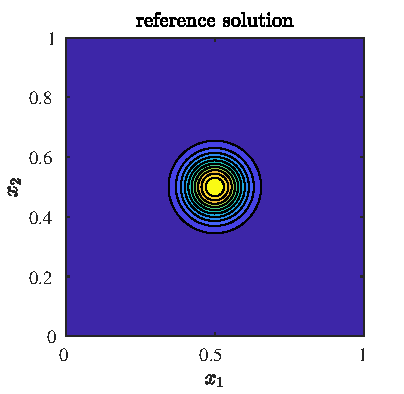
\includegraphics[]{Figures/MeshAdapt2D_ReferenceSol} & 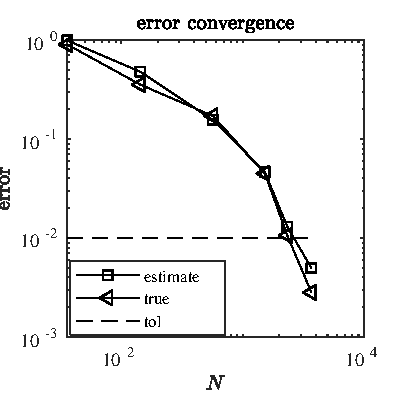
\includegraphics[]{Figures/MeshAdapt2D_ErrConv} \\
		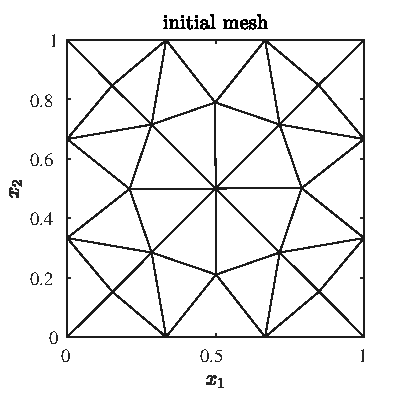
\includegraphics[]{Figures/MeshAdapt2D_InitMesh} & 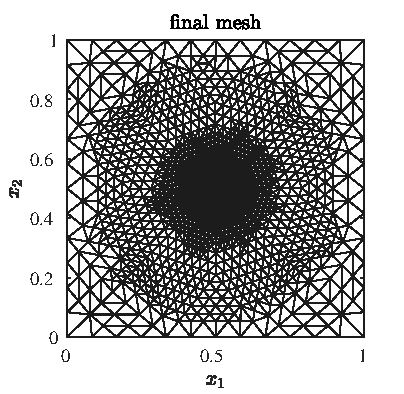
\includegraphics[]{Figures/MeshAdapt2D_FinalMesh}\\
%		\includegraphics[]{Figures/MeshAdapt2D_2_ErrEst} &\includegraphics[]{Figures/MeshAdapt2D_2_TrueErr} \\
	\end{tabular}
	\caption{Mesh adaptivity -- two-dimensional case}
	\label{fig:MeshAdaptivity2D}
\end{figure}

\begin{figure}[t]
	\centering
	\begin{tabular}{cc}
		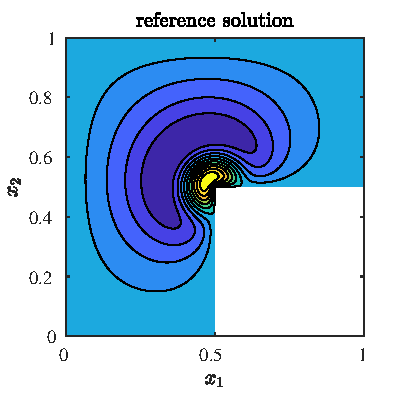
\includegraphics[]{Figures/MeshAdapt2D_2_ReferenceSol} & 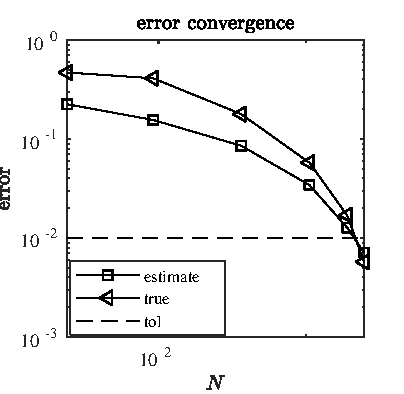
\includegraphics[]{Figures/MeshAdapt2D_2_ErrConv} \\
		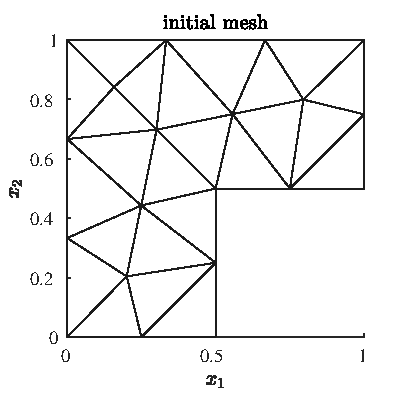
\includegraphics[]{Figures/MeshAdapt2D_2_InitMesh} & 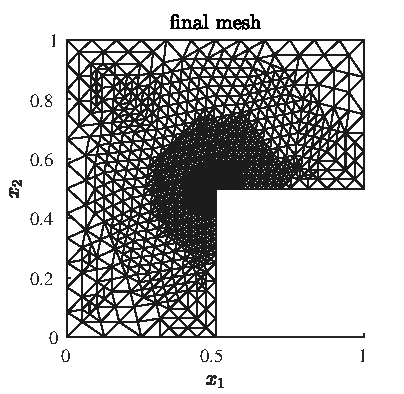
\includegraphics[]{Figures/MeshAdapt2D_2_FinalMesh}\\
%		\includegraphics[]{Figures/MeshAdapt2D_2_ErrEst} &\includegraphics[]{Figures/MeshAdapt2D_2_TrueErr} \\
	\end{tabular}
	\caption{Mesh adaptivity -- two-dimensional case}
	\label{fig:MeshAdaptivity2D_2}
\end{figure}

\subsection{Bayesian inverse problems}

Let us consider the following one-dimensional elliptic equation
\begin{equation}
\begin{aligned}
	-\frac{\dd}{\dd x}\big(e^{\kappa} \frac{\dd u}{\dd x}\big) &= f, &&\text{in } (0,1),\\
	u &= 0, &&\text{on } \{0, 1\},
\end{aligned}
\end{equation}
and the inverse problem of retrieving the field $\kappa \in \LL^2(0, 1)$ given synthetic noisy observations of the solution $u$ corresponding to a true field $\kappa^*$. First, we consider a case where information on $\kappa$ is available beforehand. In particular, we assume that $\kappa$ has the form
\begin{equation}\label{eq:fieldInfo}
	\kappa(x) = \begin{cases}	
				\log(1 + \kappa_1), & \mbox{if } x \in I_1, \\
				\log(1 + \kappa_2), & \mbox{if } x \in I_2, \\	
				0 & \mbox{otherwise},
				\end{cases}
\end{equation}
where $\kappa_1$, $\kappa_2$ are real scalars and $I_1$, $I_2$ are the intervals $(0.2, 0.4)$ and $(0.6, 0.8)$ respectively. Fixing a standard Gaussian prior on both parameters $\kappa_1$ and $\kappa_2$ we are able to compute the posterior distribution corresponding to both the deterministic and probabilistic forward models. In particular, we vary the number of elements $N$ in the set $\{20, 40, 80, 160\}$, thus studying the effects of numerical errors on the numerical posterior distribution. Observations are obtained from a reference solution evaluated at four equispaced points in the interior of $(0, 1)$ each corrupted by an additive source of noise $\epl \sim \mathcal N(0, 10^{-4})$. The posterior distributions are obtained with Metropolis--Hastings initialised near the true value of $(\kappa_1, \kappa_2)$ and ran as explained in \cref{sec:inverseproblems}, with 240 parallel chains employed for the probabilistic forward model. Results are shown in \cref{fig:BayesFin}, where \todo

In a second experiment, we consider the same exact field $\kappa^*$ and observation model, but without the additional information encoded in \eqref{eq:fieldInfo}.

\begin{figure}[t]
	\centering
	\begin{tabular}{cc}
		\includegraphics[]{Figures/Bayes_Fin_Det} & \includegraphics[]{Figures/Bayes_Fin_Prob} \\
	\end{tabular}
	\caption{Bayesian inverse problem -- finite dimensional case.}
	\label{fig:BayesFin}
\end{figure}


%\subsubsection*{L-shaped domain}
%We solve
%\begin{equation}
%\begin{aligned}
%	-\nabla \cdot (\kappa \nabla u) &= f, &&\text{in } D,\\
%	u &= 0, &&\text{on } \delta D,
%\end{aligned}
%\end{equation}
%where $D = (0, 1)^2$ domain and where $\kappa$ is given by
%\begin{equation}
%	\kappa(x) = \begin{cases} 0.1 &\mbox{if } x \in D_1,\\
%	 						  2.5 &\mbox{if } x \in D_2,\\
%	 						  1.3 &\mbox{otherwise},	
%				\end{cases}
%\end{equation}
%where $D_1$ and $D_2$ are the circles with radius $\sqrt{0.025}$ centred in $(0.25, 0.25)$ and $(0.75, 0.75)$


\bibliographystyle{siam}
\bibliography{../../anmc}
\end{document}